%==============================================================================
%== template for LATEX poster =================================================
%==============================================================================
%
%--A0 beamer slide-------------------------------------------------------------
\documentclass[final]{beamer}
\usepackage[orientation=portrait,size=a0,
            scale=1.1         % font scale factor
           ]{beamerposter}
           
\geometry{
  hmargin=2.5cm, % little modification of margins
  papersize={60cm,141cm}
}


%
\usepackage[utf8]{inputenc}

\linespread{1.15}
%
%==The poster style============================================================
\usetheme{sharelatex}

%==Title, date and authors of the poster=======================================
\title
%[Super Conference, 1 - 10 July 2013, New York, USA] % Conference
[Neural and Cognitive Computation Poster Session, Dec 30, Xuetang 117]
{ % Poster title
Temporal Coding using the Response Properties of Spiking Neurons
}

\author{ % Authors
[Team 17] Guosai Wang, Han Shen
}
\institute% General University
{
Institute for Interdisciplinary Information Sciences, Tsinghua University
%\inst{1} Very Large University, Neverland\\[0.3ex]
%\inst{2} Other University, Neverland\\[0.3ex]
%\inst{3} Yet Another University, Neverland
}
\date{\today}



\begin{document}
\begin{frame}[t]
%==============================================================================
\begin{multicols}{2}
%==============================================================================
%==The poster content==========================================================
%==============================================================================

\section{Introduction}


In biological neurons, the timing of a spike depends on the timing of synaptic currents, in a way that is classically described by the Phase Response Curve. This has implications for temporal coding: an action potential that arrives on a synapse has an implicit meaning, that depends on the position of the postsynaptic neuron on the firing cycle. Here we show that this implicit code can be used to perform computations. Using theta neurons, we derive a spike-timing dependent learning rule from an error criterion. We demonstrate how to train an auto-encoder neural network using this rule.

\section{Model Description}

\subsection{The Theta Neuron}

\begin{equation}
\label{theta_model}
	\frac{d\theta}{dt} = (1-\cos \theta) + \alpha I (1 + \cos \theta)
\end{equation}
The theta neuron is described by the differential equation~\ref{theta_model}.
($\theta$: the \emph{potential} of the neuron. $I$: a variable \emph{input current}.)
The neuron is said to \emph{fire} every time $\theta$ crosses $\pi$.
The dynamics of the model can be represented on a phase circle (Figure~\ref{phase_circle}).

\begin{figure}
\centering
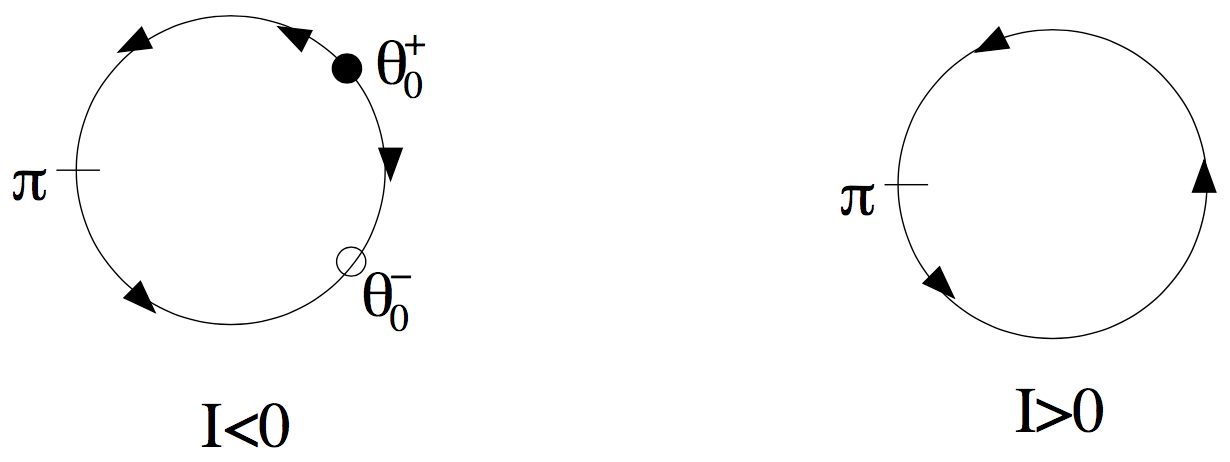
\includegraphics[width=0.6\columnwidth]{phase_circle}
\caption{
\textbf{Phase circle of the theta model.}
The neuron fires every time $\theta$ crosses $\pi$.
For $I < 0$ there are two fixed points: An unstable point $\theta_0 = \arccos\frac{1 + \alpha I}{1-\alpha I}$,
and an attractor (stable point) $\theta_0^- = -\theta_0^+$.}
\label{phase_circle}
\end{figure}

\subsection{Synaptic Interactions}

The input current $I$ is the sum of a constant current $I_0$ and transient synaptic currents $I_i(t)$, 
where $i \in 1..N$ indexes the synapses:
\begin{equation}
	I = I_0 + \sum_{i=1}^N I_i(t)
\end{equation}
Synaptic currents are modeled as Diracs: $I_i(t) = w_i\delta(t - t_i)$.
($t_i$: firing time of presynaptic neuron $i$. $w_i$: the weight of the synapse.)

\begin{figure}
\centering
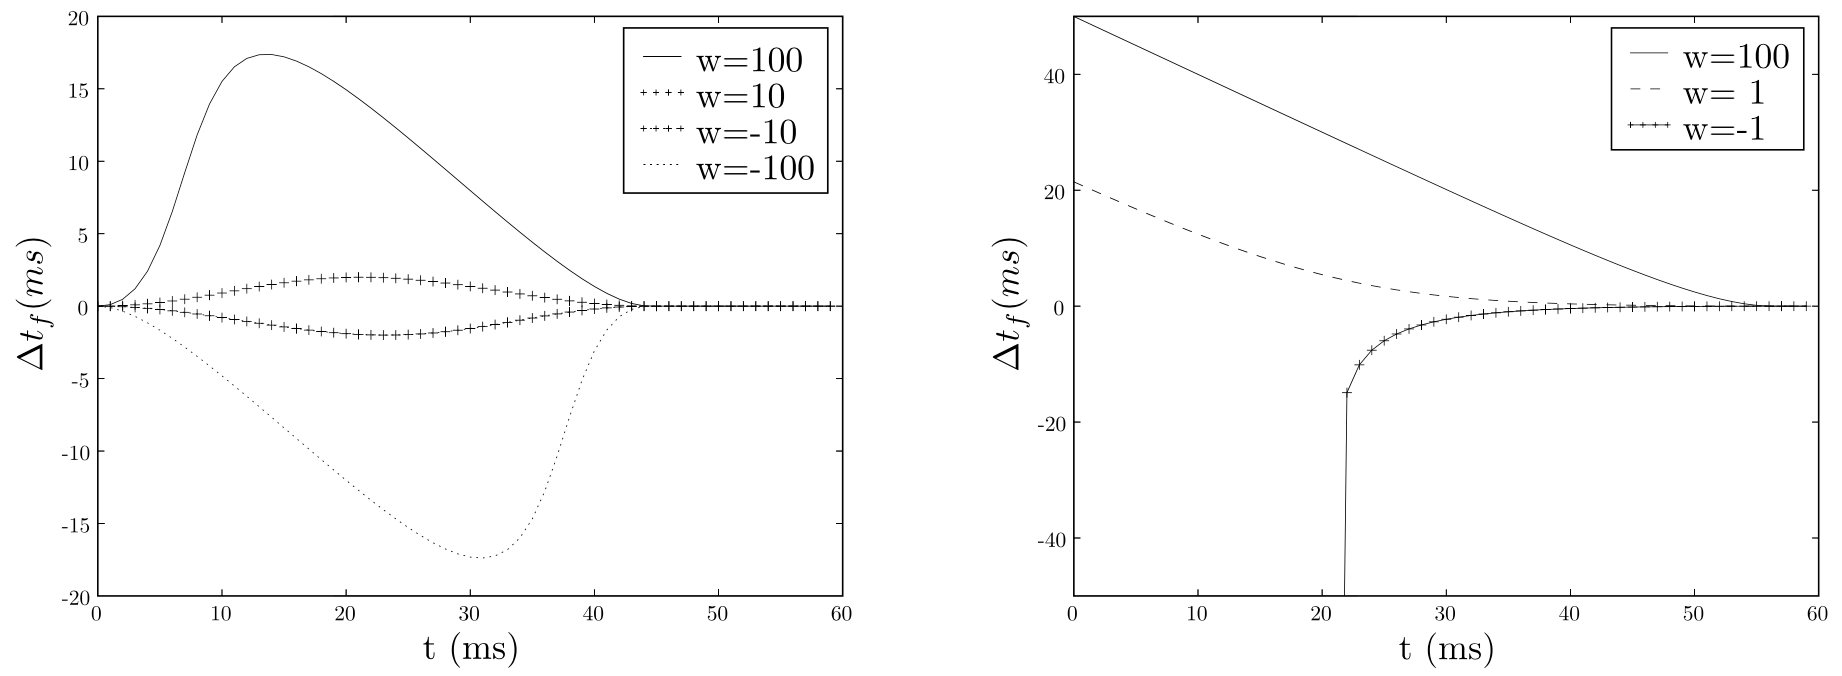
\includegraphics[width=0.98\columnwidth]{response}
\caption{\textbf{Response properties of the theta model.}
Left: For $I_0 > 0$, the neuron spikes regularly ($I_0 = 0.005$, $\theta(0) = -\pi$). 
The positive curve is called the \emph{Phase Response Curve} (PRC).
Right: Response for $I_0 < 0$.
The initial condition is slightly above the unstable equilibrium point $(I_0 = -0.005, \theta_0 = \theta_0^+ + 0.0001)$.}
\label{response}
\end{figure}
We view the curve shown in Figure~\ref{response} as the \emph{transfer function} of the neuron; 
it describes how the neuron converts input spike times into output spike times.

\begin{figure}
\centering
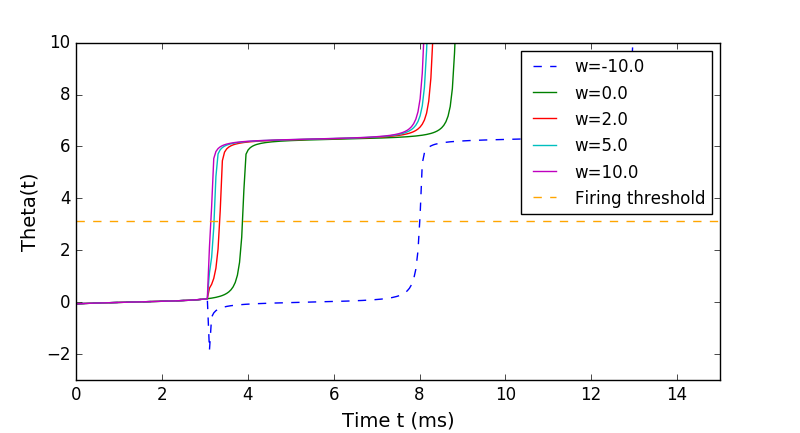
\includegraphics[width=0.52\columnwidth]{theta_t_positive_I}
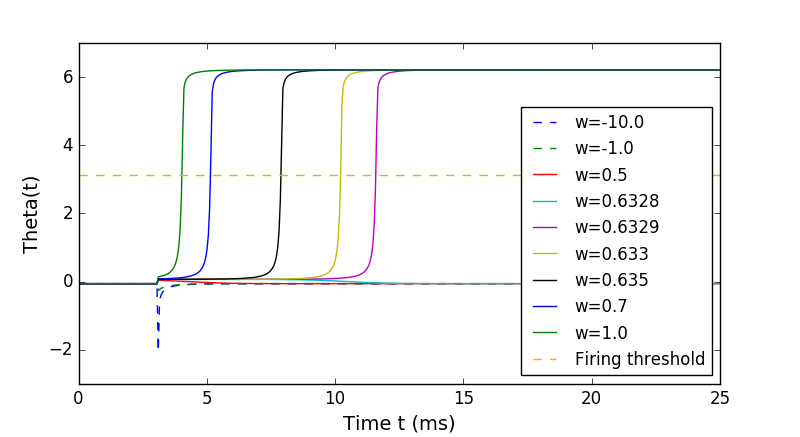
\includegraphics[width=0.52\columnwidth]{theta_t_negtive_I}
\caption{The relation between $\theta$ and $t$ given different values of $w$. 
There is only one single presynaptic neuron whose firing time is $t_i = 3.0$ ms.
Left: $I_0 = +0.01$. Right: $I_0 = -0.01$. ($\theta_0 = \theta_0^-$ and $\alpha = 0.1$ in both subfigures.)}
\label{theta_t_negtive_I}
\end{figure}

\subsection{Learning Rule}

\textbf{Objective:} learn a set of target firing times $\bar{t}_s$.

\textbf{Loss function:} the mean squared error $E=<(t_s - \bar{t}_s)^2>$.

Gradient descent on E yields:
\begin{equation}
	\Delta w_i = -\eta \frac{\partial E}{\partial w_i} = -2\eta(t_s - \bar{t}_s)\frac{\partial t_s}{\partial w_i}
\end{equation}

Let $F$ denote the ``remaining time'', i.e., the time that remains before the neuron will fire:
\begin{equation}
\label{F_t}
	F(t) = \int_{\theta(t)}^\pi \frac{d \theta}{(1-\cos \theta) + \alpha I (1 + \cos \theta)}
\end{equation}

But $I$ is not continuous. Let $t_j$ denote the time of arrival of the action potential on synapse $j$. 
Let $\theta_j^-$ (resp. $\theta_j^+$) denote the potential before (resp. after)  the synaptic current:
\begin{equation}
\left\{ \begin{array}{ll}
 \theta_j^- &= \theta(t_j^-) \\
\theta_j^+ &= \theta(t_j^+) = \theta_j +  (1 - \cos \theta_j^-) +\alpha w_j (1 + \cos \theta_j^-) 
  \end{array} \right.
\end{equation}

Rewrite Equation~\ref{F_t} on the intervals where the integrand is continuous:
\begin{equation}
	F(t_i) = \sum_{j \geq i}\int_{\theta_j^+}^{\theta_{j+1}^-} \frac{d \theta}{(1-\cos \theta) + \alpha I (1 + \cos \theta)}
\end{equation}

So the partial derivative of the spiking time $t_s$ is:
\begin{align}
\frac{\partial t_s}{\partial w_i} 
&= \frac{\partial F}{\partial \theta_i^+} \frac{\partial \theta_i^+}{\partial w_i} + \sum_{j > i} (
\frac{\partial F}{\partial \theta_j^+} \frac{\partial \theta_j^+}{\partial w_i} + 
\frac{\partial F}{\partial \theta_j^-} \frac{\partial \theta_j^-}{\partial w_i})\\
&\approx \frac{\partial F}{\partial \theta_i^+} \frac{\partial \theta_i^+}{\partial w_i}\\
&= -\frac{1+\cos \theta_i^- \alpha} {(1 - \cos \theta_i^+) + \alpha I_0(1 + \cos \theta_i^+)}
\end{align}
where the approximation derives from the lack of \emph{a priori} information on the distribution of $t_j$ given on $t_i$.\\
\textbf{Learning rule:}
\begin{equation}
\Delta w_i =
\left\{ \begin{array}{lr}
 -2\eta (t_s - \bar{t}_s) \frac{\partial t_s}{\partial w_i} & \text{if } 0 < - \frac{\partial t_s}{\partial w_i}  < C\\
2\eta (t_s - \bar{t}_s) C & \text{otherwise}
  \end{array} \right.
\end{equation}

\section{Auto-encoder Network Evaluation}

Predicting neural activities has been proposed as a possible role for spike-timing dependent learning rules. 
We train a network to predict its own activities using the learning rule derived above. 
A time-delayed version of the input (echo) is used as the desired output (see Figure~\ref{auto_encoder}). 
The network has to find a representation of the input that minimizes mean squared reconstruction error.

\begin{figure}
\centering
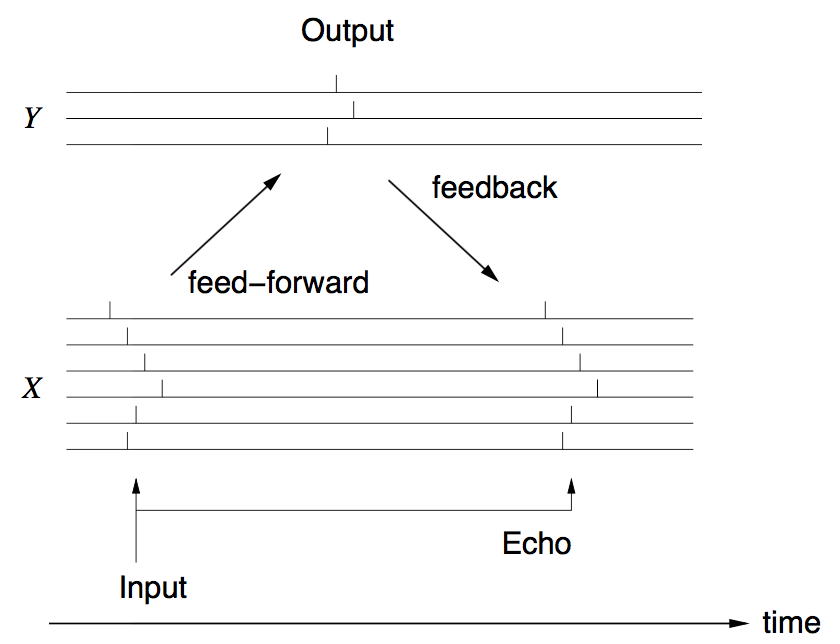
\includegraphics[width=0.5\columnwidth]{network}
\caption{The auto-encoder network tries to reconstruct the input spikes at target firing times (the echo of the input burst).
}
\label{auto_encoder}
\end{figure}

Three populations of neurons: input population $X$, which represents the input with spike times;
output population $Y$, which is activated by neurons in $X$;
reconstruction population $X'$, which reconstructs the input (with a delay).
The learning rule updates the feedback connections $(w_{ij})$ from $Y$ to $X'$, comparing spike times in $X$ and in $X'$.

\subsection{PCA of a Gaussian Distribution}

\begin{figure}
\centering
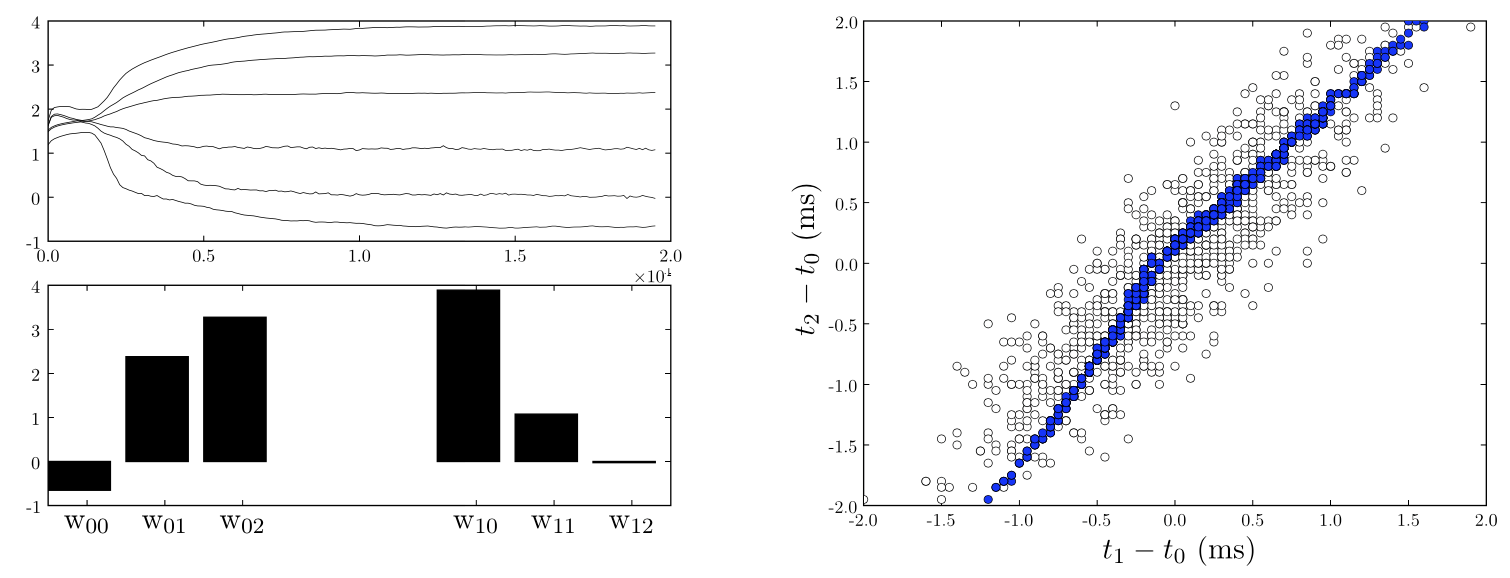
\includegraphics[width=0.98\columnwidth]{pca}
\caption{\textbf{Principal Component Analysis of a 2D Gaussian distribution.} The input vector was encoded in the relative spike times of three input neurons. The 3-2-3 network found a 1D representation of a 2D variable, that minimizes the mean-squared reconstruction error.}
\label{pca_gaussian}
\end{figure}

\subsection{Encoding Natural Images}

An 256-64-256 encoder network was trained on the set of raw natural images. 
Raw grey values from the dataset were encoded as milliseconds.
Figure~\ref{synaptic_w} shows the synaptic weights after 100,000 trials.
The mean reconstruction error on the entire dataset was 0.25ms/pixel.

\begin{figure}
\centering
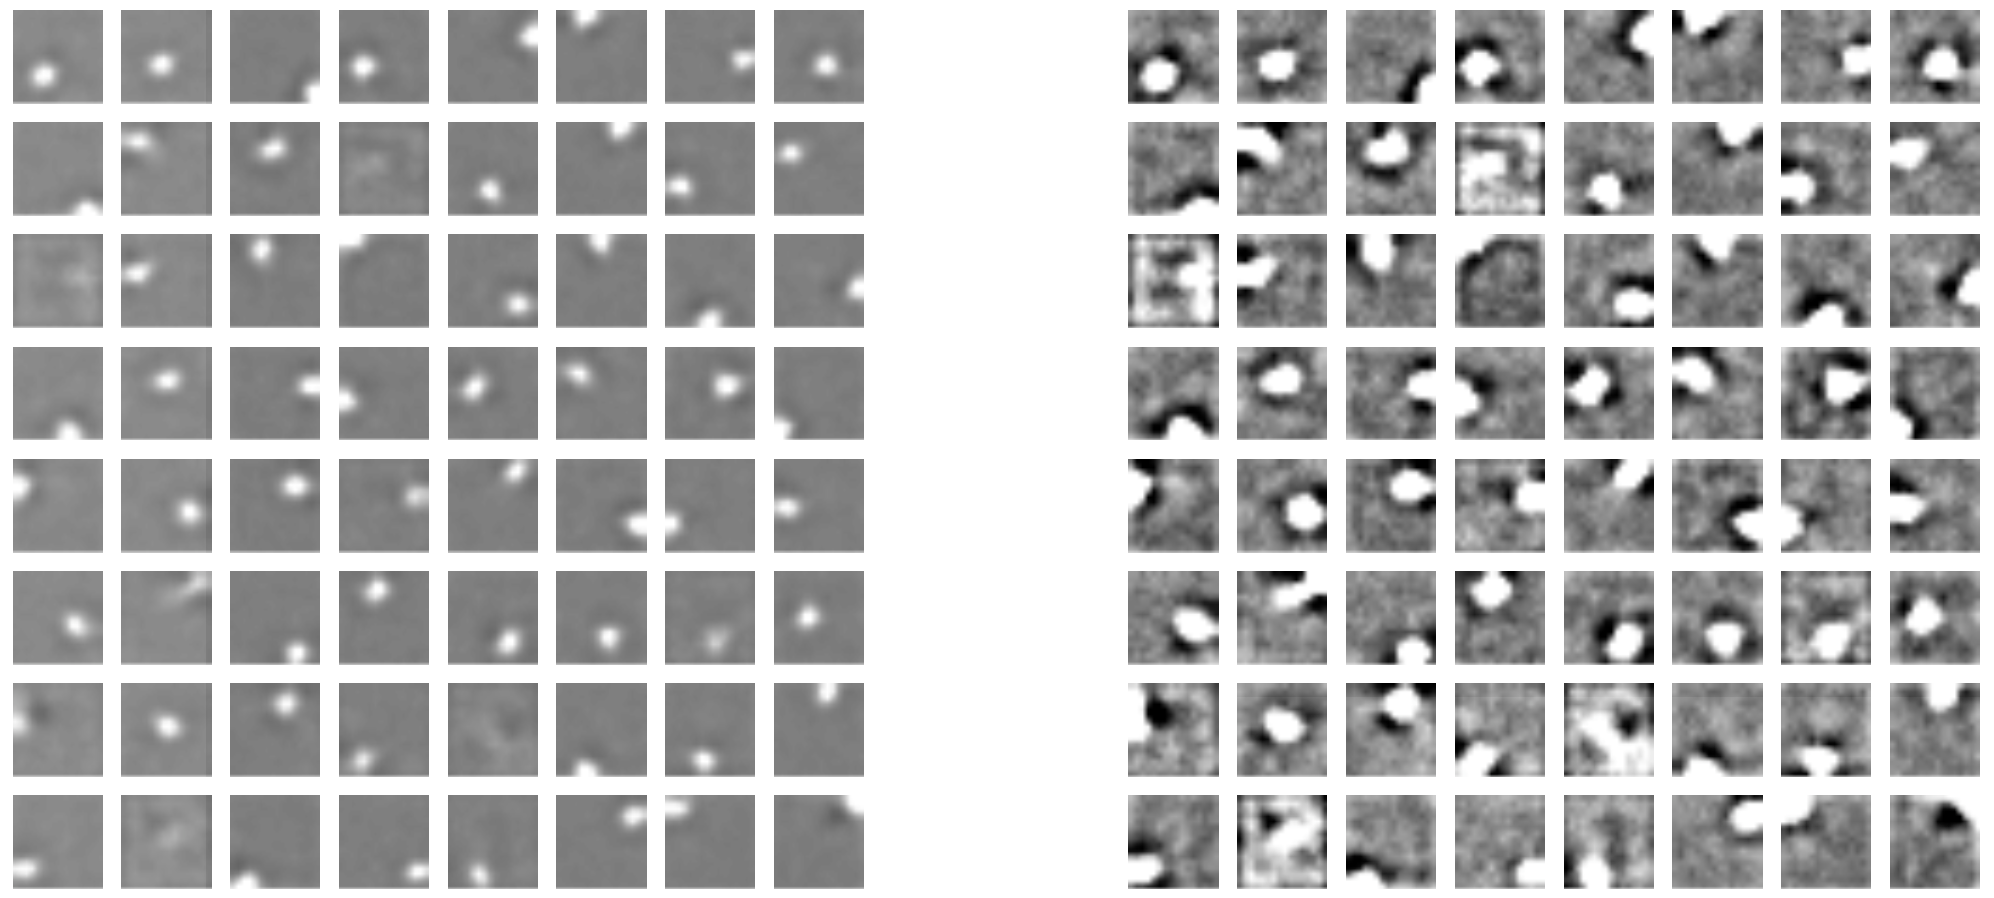
\includegraphics[width=0.8\columnwidth]{synaptic_w}
\caption{\textbf{Synaptic weights learned by the network.} 
64 neurons were trained to represent natural images patches of size 16$\times$16. 
Different grey scales are used in order to display positive and negative weights (black is negative, white is positive).}
\label{synaptic_w}
\end{figure}

The difference of amplitude between positive and negative weights results from higher sensitivity of the response curves to negative weights.

The nonlinearity of the response properties of the theta neurons causes the local-filter-shaped synaptic weights.
This nonlinearity favors sparse representations, making network perform something similar to Nonlinear PCA.




\section{Summary and Conclusions}

The dynamic response properties of spiking neurons can be effectively used as transfer functions, 
in order to perform computations (in the paper, PCA and Nature Image Encoding). 
We used theta neurons, which are of type I, and equivalent to quadratic integrate-and-fire neurons. 
Type I neurons have a PRC that is always positive. This means that spike times can encode only
positive values. In order to encode values of both signs, one would need the transfer function to change its sign around a time that codes for zero. This will be possible with more complex type II neurons, where the sign of the PRC is not constant.


%==============================================================================
%==End of content==============================================================
%==============================================================================

%--References------------------------------------------------------------------

\subsection{References}

\begin{thebibliography}{99}

\bibitem{ref1} J.~Doe, Article name, \textit{Phys. Rev. Lett.}

Schölkopf, B, Platt, J, Hofmann, T. Temporal Coding using the Response Properties of Spiking Neurons. \textit{NIPS 2006}.
\end{thebibliography}
%--End of references-----------------------------------------------------------

\end{multicols}

%==============================================================================
\end{frame}
\end{document}
